\begin{figure}[H]
    \centering
    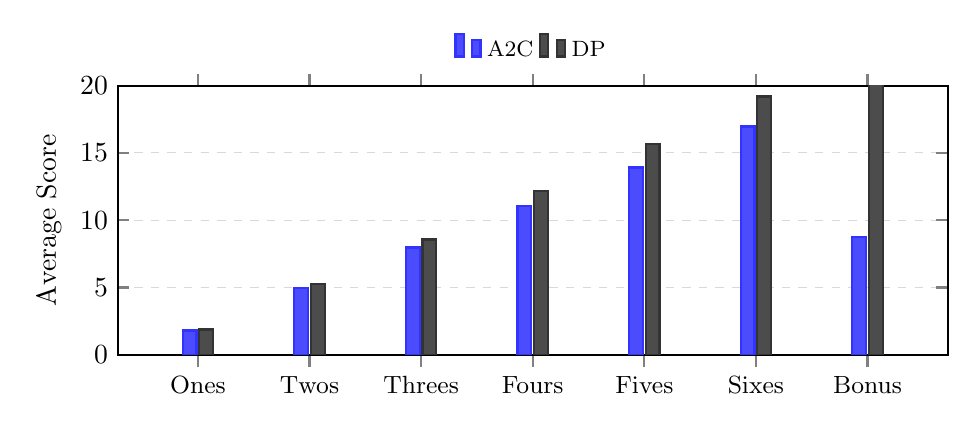
\begin{tikzpicture}
        \begin{axis}[
                ybar=1pt,
                width=\columnwidth,
                height=5cm,
                bar width=5pt,
                symbolic x coords={Ones,Twos,Threes,Fours,Fives,Sixes,Bonus},
                xtick=data,
                xticklabel style={font=\small},
                ylabel={Average Score},
                ymin=0,
                ymax=20,
                ymajorgrids=true,
                grid style={dashed,gray!30},
                legend style={
                        at={(0.5,1.05)},
                        anchor=south,
                        legend columns=4,
                        font=\footnotesize,
                        draw=none,
                        fill=none
                    },
                enlarge x limits=0.12,
                axis line style={thick},
                tick style={thick},
            ]

            % A2C
            \addplot[fill=blue!70!white, draw=blue!80!white, thick] coordinates {
                    (Ones,   1.80) (Twos,   4.96) (Threes, 7.97) (Fours,  11.08)
                    (Fives,  13.92) (Sixes,  16.97) (Bonus,  8.73)
                };

            % PPO
            %\addplot[fill=red!60!white, draw=red!80!white, thick] coordinates {
            %        (Ones,   5) (Twos,   5) (Threes, 5) (Fours,  5)
            %        (Fives,  5) (Sixes,  5) (Bonus,  5)
            %    };

            % REINFORCE
            %\addplot[fill=green!60!white, draw=green!80!white, thick] coordinates {
            %        (Ones,   5) (Twos,   5) (Threes, 5) (Fours,  5)
            %        (Fives,  5) (Sixes,  5) (Bonus,  5)
            %    };

            % DP
            \addplot[fill=black!70, draw=black!80, thick] coordinates {
                    (Ones,   1.88) (Twos,   5.28) (Threes, 8.57) (Fours,  12.16)
                    (Fives,  15.69) (Sixes,  19.19) (Bonus,  23.84)
                };

            \legend{A2C,DP}

        \end{axis}
    \end{tikzpicture}
    \caption{Upper section and bonus scores (placeholder data)}
    \label{fig:category-upper}
\end{figure}
